\section*{2.3 Método de Newton y sus variantes}

El método de Newton está basado en los polinomios de Taylor.
Suponga que $f\in C^2[a,b]$. Sea $p_0\in [a,b]$ una aproximación a $p$ tal que $f'(p_0)\neq0$ y $|p-p_0|$ "pequeño". Considere el primer polinomio de Taylor de $f(x)$ expandido en $p_0$ y evaluado en $x=p$.

\begin{equation*}
    f(p)=f(p_0)+(p-p_0)f'(p_0)+\frac{(p-p_0)^2}{2}f''(\xi(p)),
\end{equation*}

Donde $\xi(p)$ se encuentra entre $p$ y $p_0$. Dado que $f(p)=0$ esta ecuación se transforma en:

\begin{equation*}
    0=f(p_0)+(p-p_0)f'(p_0)+\frac{(p-p_0)^2}{2}f''(\xi(p)),
\end{equation*}

El método de Newton es derivado de asumir que $|p-p_0|$ es pequeño, entonces el término envolvente $(p-p_0)^2$ es mucho mas pequeño, por lo tanto: 

\begin{equation*}
    0\approx f(p_0)+(p-p_0)f'(p_0),
\end{equation*}

Resolviendo para $p$ se obtiene: 

\begin{equation*}
    p\approx p_0 -\frac{f(p_0)}{f'(p_0)}\equiv p_1,
\end{equation*}

Esto es la base para el método de Newton, el cual empieza con una aproximación $p_0$ y genera la secuencia $\{p_n\}_{n=0}^{\infty}$ con

\begin{equation*}
    p_n= p_{n-1} -\frac{f(p_{n-1})}{f'(p_{n-1})}, \ para \ n\geq 1.
\end{equation*}

La figura \ref{tab:fig3} ilustra como las aproximaciones son obtenidas utilizando tangentes. Comenzando con la aproximación inicial $p_0$, la aproximación $p_1$ es la intersección con el eje x de la linea tangente a la función $f$ en el punto $(p_0,f(p_0))$. La aproximación $p_2$ intersección con el eje x de la linea tangente a la función $f$ en el punto $(p_1,f(p_1))$ y así sucesivamente.

\begin{figure*}[h!]
\centering
  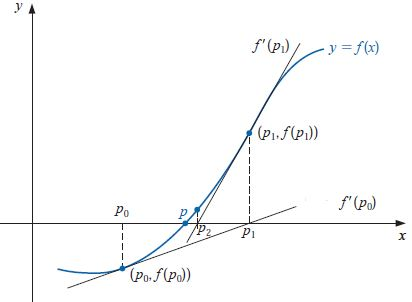
\includegraphics[width=0.6\textwidth]{Newton.JPG}
\caption{Newton}
\label{tab:fig3}
\end{figure*} 

\begin{tcolorbox}[colback=blue!15!]
\subsubsection*{Método de Newton}
Para encontrar la solución a $f(x)=0$ dada la aproximación inicial $p_0$:
\\ \\
ENTRADA aproximación inicial $p_0$; tolerancia \textit{TOL}; número máximo de iteraciones $N_0$.

SALIDA La solución aproximada \textit{p} o mensaje de falla.

PASO 1 Asigna i=1;

PASO 2 Mientras $i\leq N_0$ ejecuta los pasos 3-6.

\ \ \ \  PASO 3 Asigna $p=p_0 -\frac{f(p_0)}{f'(p_0)} $; (calcula $p_i$)

\ \ \ \  PASO 4 Si $|p-p_0|<TOL$ entonces

\ \ \ \ \ \ \ \ \ \ \ \ \ \ \ \ \ \ SALIDA (p); (proceso completado exitosamente)

\ \ \ \ \ \ \ \ \ \ \ \ \ \ \ \ \ \ ALTO.

\ \ \ \   PASO 5 Asigna $i=i+1$
    
\ \ \ \   PASO 6 Asigna $p_0=p$; (Actualiza $p_0$.)

PASO 7 SALIDA ('El método fallo después de $N_0$ iteraciones $N_0=$',$N_0$);

\ \ \ \ \ \ \ \ \ \ \ \ \ (El proceso fue exitoso.)

\ \ \ \ \ \ \ \ \ \ \ \ \ ALTO.


\end{tcolorbox}

La diferencia generada en la aproximación dada por el método de Bisección también aplicable al método de Newton. Esto es, selecciona una tolerancia $\varepsilon>0$ y construye $p_1,\dotsc,p_n$ hasta
\begin{center}
    $|p-p_0|<\varepsilon$,
\end{center}

El método de Newton es una técnica de iteración funcional con $p_n=g(p_{n-1})$ tal que 

\begin{equation*}
    g(p_{n-1})= p_{n-1} -\frac{f(p_{n-1})}{f'(p_{n-1})}, \ para \ n\geq 1.
\end{equation*}

\subsubsection*{Ejemplo}
Considere la ecuación $f(x)=cos x-x=0$ aproxima la raíz de $f$ usando el método de Newton.

\textbf{Solución}. Primero para elegir un $p_0$ adecuado partimos de la figura \ref{tab:fig4}:

\begin{figure*}[h!]
\centering
  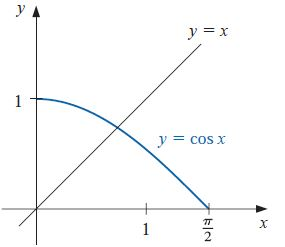
\includegraphics[width=0.6\textwidth]{NewtonE.JPG}
\caption{Newton cos x}
\label{tab:fig4}
\end{figure*} 

Para aplicar el método de Newton se necesita $f'(x)=-sinx-1$. Y se toma a $p_0=\pi/4$, se genera entonces la secuencia definida con $n\geq 1$ por:

\begin{equation*}
    p_n= p_{n-1} -\frac{f(p_{n-1})}{f'(p_{n-1})}=p_{n-1} -\frac{cosp_{n-1}-p_{n-1}}{-sinp_{n-1}-1}.
\end{equation*}

Esto da la aproximación de la tabla \ref{tab:tabla5}. Una excelente aproximación se obtiene con $n=3$. Debido a la concordancia de $p_3$ y $p_4$ se puede esperar que este resultado sea exacto para las siguientes aproximaciones. 

\begin{table}
\centering
    \begin{tabular}{||c c||}
    \hline 
    \hline
        \multicolumn{2}{c}{\textbf{Método de Newton}}\tabularnewline
        $n$ & $p_n$      \\
    \hline 
    \hline 
        0 & 0.7853981635 \\
        1 & 0.7395361337 \\
        2 & 0.7390851781 \\
        3 & 0.7390851332 \\
        4 & 0.7390851332 \\
        \hline
        \hline 
    \end{tabular}
\caption{Newton cosx}
\label{tab:tabla5}
\end{table}
